\chapter{State of The Art} \label{chap:stateoftheart}
DevOps is usually associated with different types of technologies and practices. Effectively practicing DevOps means not only to understand the cultural aspects but also the technological aspects that enabled some of its practices. \\
In this chapter an introduction to cloud computing will be presented, providing the needed context for the following section where a description of the DevOps movement is presented. After this, both a small characterization of the Portuguese startup scene and of pattern languages will be presented in order to justify some of the choices presented in the next chapters.

    \section{Cloud Computing} \label{chap:stateoftheart:sec:cloud}
    Paraphrasing \cite{Bass}, consider the need for electricity. Rather than building an entire grid and a power plant, one only needs to connect to the public network. In the common scenario, charges are calculated based on the usage amount and no special knowledge of how the network setup is needed.\\
    Clouds follow exactly the same rationale, rather than having to build/purchase the computing resources, one needs only to connect to a provider and the resources are available to be used. Charges, like in the electric grid, are calculated based on the usage and clients do not need to know how the resources are managed or setup.
        \subsection{Definition} \label{chap:stateoftheart:sec:cloud:sec:definition}
        In \cite{Mell2011}, NIST\footnote{National Institute of Standarts and Technologie} defines Cloud computing as \textit{a model for enabling ubiquitous, convenient, on-demand network access to a shared pool of configurable computing resources (e.g., networks, servers, storage, applications, and services) that can be rapidly provisioned and released with minimal management effort or service provider interaction.}

        NIST also defines the following essential characteristics of cloud computing:

        \begin{itemize}
            \item \textbf{On-demand self-service} : A consumer can unilaterally provision computing capabilities, e.g. server time and network storage, automatically without requiring human interaction with each service provider \cite{Mell2011}.
            \item \textbf{Broad network access} :  Users must be allowed to access resources through standard mechanism \cite{Mell2011}.
            \item \textbf{Resource pooling} : A multi-tenant model should be used in order to serve multiple users. Resources are allocated dynamically meaning that users do not know were, physically, the allocated resources are \cite{Garrison2012}
            \item \textbf{Rapid elasticity} : Resources can be elastically allocated or deallocate. This should be done automatically \cite{Mell2011}.
            \item \textbf{Measured service} : The usage of resources should be measured providing transparency in the provider-client relation \cite{Mell2011}.
  	    \end{itemize}

        \subsection{Delivery methods} \label{chap:stateoftheheart:sec:cloud:sec:deliverymethods}
          In regards to their accessibility, it is common to identify three main categories of clouds \cite{Zhang2010} :
        	\begin{itemize}
            	\item \textbf{Public Clouds} : Public clouds are a pool of resources hosted by cloud providers who rent them to the general public. This resources can be accessed over the Internet and are shared among users.

    		      \item \textbf{Private Clouds} : Private clouds are usually administered and used by the same organization. Alternatively a third party can also be hired to manage the resources. The main difference between public and private clouds is the usage of the resources. Private clouds resources are only used by one company as opposed to public clouds were resources are shared.

              \item \textbf{Hybrid Clouds} : Hybrid clouds combine both the private and public concepts. When using a hybrid clouds approach, infrastructure is divided by the two types of clouds meaning that some modules may be hosted in the private space and others on the public one.

              \item \textbf{Virtual Private Cloud} : Virtual private clouds are an alternative to private clouds. This type of cloud are essentially a public cloud that \textit{leverages virtual private network (VPN) technology} \cite{Zhang2010} allowing users to combine characteristics of both public clouds and private clouds.
    		\end{itemize}

      \subsection{Service Levels} \label{chap:stateoftheheart:sec:cloud:sec:servicelevels}
  		In terms of service levels cloud computing can be classified in regard to the provided abstraction. The main categories are the following \cite{Vaquero2008} :
  		\begin{itemize}
  			\item \textbf{SaaS} - Software as a Service (SaaS) gives users access to a platform usually through a web client without the need to  download or install software. The user is able to use the provided software instantly and virtually everywhere.\linebreak Applications of this model include messaging software, email services, collaborative platforms, etc.
 				\item \textbf{PaaS} - Platform as a Service (PaaS) allows its users to quickly deploy applications with little to no configuration. In this type of platform environments are usually setup previously or configurable. PaaS users should nevertheless expect only to be able to deploy applications or software supported by the provider.
  			\item \textbf{IaaS} - Infrastructure as a Service (IaaS) represents the lowest abstraction made available by cloud providers. In this model the user is able to configure and access a machine directly without constraints. This machine, usually a virtual server managed by the provider, can be configured and maintained by the user.\linebreak This model is used when applications are complex and therefore need complex configurations.
  		\end{itemize}

  		\subsection{Benefits} \label{chap:stateoftheheart:sec:cloud:sec:benefits}
  			The main advantages of cloud computing for its users can be summarized as following:
  			\begin{itemize}
  				\item \textbf{Monetary Efficiency} - Cloud providers allow users to keep their resources to the needed minimum. By allowing users to quickly and easily increase/decrease the allocated resources amount and billing clients only for the resources used, cloud providers are good way to save money and spend only the needed amount \cite{Garrison2012,Mell2011}.
  				\item \textbf{Scalability} - usually through a public API of some kind most cloud providers allow for the quick increase or reduction of resources \cite{Mell2011}. This enables businesses to quickly go from zero to millions of users with minimum overhead. Additionally, because processes related with the management and configuration of cloud servers can be automated, it is usually possible to manage large systems with small teams \cite{Loukides2012}.
  	    	\item \textbf{Maintainability} - Cloud Providers are responsible for the maintenance of all the hardware and infrastructure aspects. Cloud computing users therefore do not need to worry about updating the hardware or maintaining the physical infrastructure. This enables users to focus their resources in improving their product rather than improving the structure that supports it \cite{Garrison2012}.
  			\end{itemize}

	\section{DevOps} \label{chap:stateoftheart:sec:devops}
      In \textit{Why DevOps Is Like An Onion} \cite{DaveSayers2013}, Dave Sayers chooses to use the analogy of peeling an onion, with each layer representing a different concept, in order to describe DevOps. Further developing upon his initial idea, in this section, we will try to introduce DevOps using that same analogy.

      \subsection{The cultural layer} \label{chap:stateoftheart:sec:devops:sec:culture}
      Looking at some of the first DevOps efforts we see that a lot of them aimed to create a better articulation between Developers and Operations \cite{Debois2008,Allspaw}.\\
      Being two distinct departments with different work methodologies and objectives, this meant that some cultural changes had to happen in order for the two departments to be able to create a common understanding of each other worlds \cite{Allspaw}.\\
      The main cultural values associated with DevOps are, as a result, values that promote cooperation and communication. These are some of the ones that we identified:
      \begin{itemize}
          \item Respect \cite{Davis2015,Allspaw}
          \item Trust \cite{Huttermann2012}
          \item Collaboration \cite{Davis2015}
          \item Sharing \cite{Willis2010}
      \end{itemize}

      \subsection{The methodology layer} \label{chap:stateoftheart:sec:devops:sec:methodology}
      The DevOps movement does not define a specific methodology. Nevertheless, when we look for instance at CAMS \ref{chap:stateoftheart:sec:devops:sec:definition} or at some of the practices like \textit{Continuous Deployment} it becomes clear that, although a methodology is not defined, the one chose should enable an iterative and continuous improvement focused approach.

      \subsection{The practices layer} \label{chap:stateoftheart:sec:devops:sec:practices}
      Broadly speaking, DevOps practices gravitate around the automation of processes. From the setup of environments on the developers machine, up to the deployment phase, the capacity to automate repetitive tasks is a key feature of DevOps.
      Common practices associated with the DevOps movement include:
      \begin{itemize}
        \item \textbf{Continuous Integration} - Regular integration of software helps discover risks associated with the integration of the software. \cite{And2015}
        \item \textbf{Continuous Deployment} - Deploying often means that less functionality are deployed each time. This makes deployments more manageable and in turn safer \cite{Allspaw}.
        \item \textbf{Continuous Monitoring} - Continuously monitoring infrastructure and applications allows for the early detection of bugs \cite{Cukier2013}. It can also be a way to identify areas that can be improved \cite{Willis2010}
        \item \textbf{Defining infrastructure as code} - By defining infrastructure as code it is possible to increase reliability and consistency \cite{Loukides2012}.
        \item \textbf{Using feature Flags} - Feature flags are special flags that toggle features on and off.  This can improve error handling by allowing faulty features to be turned off. Feature flags also enable more complex schemes of operation where certain functionality are launched, but are not displayed or are displayed just to certain users. Once it is observed that the new functionality works, the flag can be turned on and the new functionality is available \cite{Bass}.
        \item \textbf{Others} - As we will see in \ref{chap:stateoftheart:sec:devops:sec:definition} there can be a great number of practices that can be considered DevOps practices.
      \end{itemize}

      \subsection{The tool layer} \label{chap:stateoftheart:sec:devops:sec:tools}
      Tools allow for some practices to be more effective. In this section we will present some of the existent categories of tools. This categories are presented in \cite{Labs} and are currently being maintained and increased by the DevOps community:
      \begin{multicols}{3}
        \begin{itemize}
            \item Source Control Management (SCM)
            \item Continuous Integration (CI)
            \item Deployment management
            \item Cloud platform and infrastructure
            \item Monitoring
        \end{itemize}
        \begin{itemize}
            \item Repository Management
            \item Infrastructure Provisioning
            \item Release management
            \item Logging
            \item Security
        \end{itemize}
        \begin{itemize}
            \item Build
            \item Testing
            \item Containerization
            \item Collaboration
            \item Database Management
        \end{itemize}
      \end{multicols}
\pagebreak
      \subsection{The full onion} \label{chap:stateoftheart:sec:devops:sec:onion}
        \begin{wrapfigure}{R}{0.4\textwidth}
            \center
            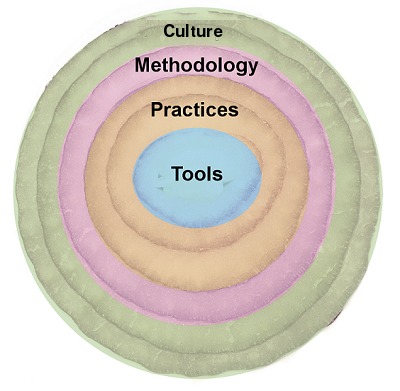
\includegraphics[width=0.8\linewidth]{onion}
            \caption{The DevOps onion \cite{DaveSayers2013}}
            \label{fig:onion}
        \end{wrapfigure}
        As it was stated by Paul Hammon and John Allspawn at their \textit{10+ Deploys Per Day: Dev and Ops Cooperation at Flickr} \cite{Allspaw} presentation, tools and processes alone are not enough and the cultural change should be the first step to take towards DevOps. \\
        Because of this, the outermost layer in the onion (fig. \ref{fig:onion}) represents the most important layer and without \textit{peeling} it will not be possible to take advantage of the  inner layers \cite{Allspaw}.

        \subsection{A DevOps definition} \label{chap:stateoftheart:sec:devops:sec:definition}
        DevOps vastness can be seen in the enormous amounts of tools categories identified in \ref{chap:stateoftheart:sec:devops:sec:tools} related with DevOps.\\
        As one might expect from this vastness of areas that DevOps touches, there are still difficulties to properly define DevOps. In order to reduce this lack of definition, we will use throughout this thesis a conjugation of two definitions for DevOps.\\
        The first definition is from \textit{DevOps: A Software Architect's Perspective} \cite{Bass} and it states that: \\
        \\
        \textit{DevOps is a set of practices intended to reduce the time between committing a change to a system and the change being placed into normal production, while ensuring high quality.} \\
        \\
        We chose this definition because it allows to easily classify something as being DevOps or not, i.e. one would only have to ask himself if a practice or cultural aspect will allow for the reduction of time since committing a change until that change is in production, if it does, then it is DevOps. Nevertheless, we find this definition to be a bit empty in the sense that by only reading it one would not be aware of the aspects that are associated with Devops. As a workaround for this problem we use a second definition based on the CAMS acronym.\\
        The CAMS acronym \cite{Willis2010} defines DevOps as being a \textbf{C}ultural movement where \textbf{A}utomation and continuous \textbf{M}easurement of processes and people are promoted and where the later can serve as an input for the \textbf{S}haring of problems and new ideas. As new ideas appear to solve the identified problems, new measurements can be made to further identify problems further improving the overall process.

        \subsection{DevOps Benefits}
        In a recent study \cite{Elliot2015} the following benefits were identified:
  		  \begin{itemize}
            \item DevOps projects are believed to accelerate in 15\%-20\% the ability to delivery of capabilities to the client
            \item Adopting DevOps allows business to practice Continuous Delivery.
            \item The average cost of a critical application failure per hour is \$500,000 to \$1 million (DevOps can help reduce application failures).
            \item The average cost percentage (per year) of a single application's development, testing, deployment, and operations life cycle considered wasteful and unnecessary is 25\% (DevOps can help automate some repetitive tasks and by doing so reducing some of the waste associated with those tasks)
  		  \end{itemize}

      \subsection{Patterns}
      Some previous progress has already been made regarding the identification of DevOps related patterns. We will summarize this progress by listing the identified patterns and briefly describing them:
      \begin{itemize}
        \item \textbf{Store Big Files in Cloud Storages}\cite{Cukier2013} - Instead of creating and managing a system to store large files, or storing them in database columns, store them in a Cloud Storage\footnote{A storage system provided by a cloud provider.}
        \item \textbf{Queue based solution to process asynchronous jobs}\cite{Cukier2013} - When there are tasks that take a long time to complete but users still expect a quick response, create a new Job instance in a queueing service and then have a service performing those tasks. When finished, post the result of that Job somewhere acessible to the user and notify the user that the task is done.
        \item \textbf{Prefer PaaS over IaaS}\cite{Cukier2013} - For non technology companies, PaaS is usually preferable because it will give them lot of functionality without the need for configuration. This will allow them to simply focus on their core business.
        \item \textbf{Load Balancing Application Server with memcached user sessions}\cite{Cukier2013} - Use a load balancer in front of your application servers. This severs will handle sessions using memcached which means that if a application server goes down or if a new application server is needed, it will be able to use the user session.
        \item \textbf{Email delivery}\cite{Cukier2013} - Rather than implementing your own SMTP solution, use cloud mail delivery services which provicde REST API's to send emails.
        \item \textbf{Logging}\cite{Cukier2013} - Having multiple servers you need a way to consolidate your application logs. In order to do so, you should use a cloud based log service.
        \item \textbf{Realtime User Monitoring (RUM)}\cite{Cukier2013} - Monitor user behaviour in order to find possible bugs or errors.
        \item \textbf{The isolation by containerization pattern} \cite{Sousa2015} - \textit{Use a container to package the applications and its dependencies and deploy the service within it}.
        \item \textbf{The discovery by local reverse proxy pattern} \cite{Sousa2015} - \textit{Configure a service port for each service, which is routed locally from each server to the proper destination using a reverse proxy.}
        \item \textbf{The orchestration by resource offering pattern} \cite{Sousa2015} - \textit{Orchestrate services in a cluster based on each host’s resource-offering announcements.}

      \end{itemize}


  	\section{The Portuguese startup scene} \label{sec:stateoftheart:sec:portuguesestartupscene}
    Motivated by a recent investment in innovation and entrepreneurship, Portugal startups have been growing their position in the global startup scene \cite{Coleman2015}.

    A study from 2015 \cite{StartupEuropePartnership2015} in which the Portuguese startup scene was analyzed, revealed that there were already 40 technology scaleups \footnote{Scaleups are companies that raised more than \$1M funding (since foundation) and had at least one funding event in the last five-year period } operating in Portugal at the time. The same study stated that this startups were able to raise a large portion of the received investment from international investors indicating, therefore, that the reach and scale of this startups was broader than just the national arena. Additionally, it is also indicated in the study that Porto and Lisbon are the main centers of innovation, encompassing 70\% of the total of existing scaleups. In addition to the scaleups identified other smaller scale startups exist. Some of this startups are currently being incubated in incubators around the country like UPTEC \footnote{Science and Technology Park of University of Porto} and Startup Lisboa. This incubators had, at the time of this study more than 300 companies \cite{Uptec,StartupLisboa} under their wing.


    \section{A pattern language} \label{sec:stateoftheart:sec:patterns}
    Cristopher Alexander wrote \textit{A Pattern Language}\cite{alexander1977pattern} in 1977 and in doing so, introduced the idea of representing knowledge on the form of a pattern language. Since then, pattern languages have been used in several areas \cite{Meszaros1998} including software development where they were used to describe common architectural solutions \cite{kircher2013pattern} or recurring software design choices \cite{johnson1995design}.  \\
    A pattern is a recurring solution to a problem that lives inside a specific context \cite{Meszaros1998}. Pattern languages are \textit{collections of patterns that are related to each other by virtue of solving the same problems or parts of a solution to a larger, partitioned problem.} \cite{Meszaros1998}.\\
    There are some key characteristics that should be taken in consideration when writing patterns. In \textit{A pattern language for pattern writing} \cite{Meszaros1998}, some of this characteristics are presented in a form of patterns themselves, they can be summed up as follows:
    \begin{itemize}
      \item patterns should identify a pattern \textbf{user} operating in a \textbf{context}. This pattern user should have and identified \textbf{problem} that he solves using a \textbf{solution} that takes into consideration some of the constraints defined by the context.
      \item patterns should be easy to read and understand and should not force the reader to read the entire pattern multiple times in order understand it.
    \end{itemize}
    Because patterns represent a way to share recurring solutions to a problem \cite{Meszaros1998}, pattern languages help reduce re-discovery and re-invention of concepts and functionality as well as \textit{avoiding common pitfalls that are learned from experience} \cite{Schmidt1995}.
